\documentclass[10pt, a4paper]{report}
\usepackage[utf8]{inputenc}
\usepackage{graphicx}
\usepackage{nomencl}
\usepackage{makeidx}

\makenomenclature
\title{{\Huge Interoperatability in Health Information Systems} \\ Report \\ Specialization Project \\ TDT4501}
\author{Kenneth Børtveit}
\begin{document}
\maketitle
\tableofcontents
\listoffigures
\listoftables
\printnomenclature
%Compile, then run this command to make the nomenclature
%makeindex  filename.nlo -s nomencl.ist -o filename.nls
%Then compile a couple of times.
\begin{abstract}

\end{abstract}
\chapter{Introduction}
\section{Research Questions}
What kind of tools and method of approach is necessary for optimeizing interoperability in developing countries?

\part{Litterature}
\chapter{Interoperatability}
\chapter{Datawarehouse}
\chapter{Integration}
\chapter{Transition Strategy}
\section{System Migration \cite{2} \cite{8}}
\subsection{Initiation}
Who is the initiators and how does this impact the choice of system.
\subsection{Implementation}
\subsubsection{What characterizes a successful implementation}
\subsection{Cut-Over}
\subsubsection{Evolutionary vs. Revolutionary}
\subsection{Migration Methods}
\subsubsection{The Big Bang}
\subsubsection{Forward Migration}
\subsubsection{Backwords Migration}
\subsubsection{The Chicken Little Strategy}
\subsubsection{The Butterfly Methodology}
 
\part{Empirical}
\chapter{Context}
\begin{figure}
\centering
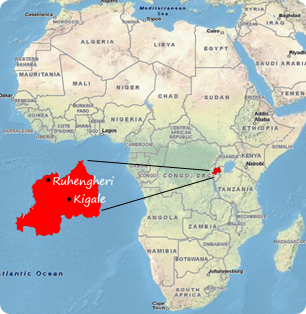
\includegraphics[width=12cm]{empirical/images/context_map_rwanda}
\label{context_map_of_rwanda}
\caption{Rwanda in the World \cite{14}}
\end{figure}
In the center of Africa we find Rwanda. A very small country, only \(26338 km^2\). This would be about 7\% of Norway. 
Their population is estimated to be around 12 million wich makes it about 420 people pr. square kilometer. 
Rwanda is made up of 5 provinces, east, west, north, south and Kigali. 
Each province is again divided into districts and there is a total of 30 districts. Under districts there is a total of 416 sectors\cite{1}.
\begin{figure}
\centering
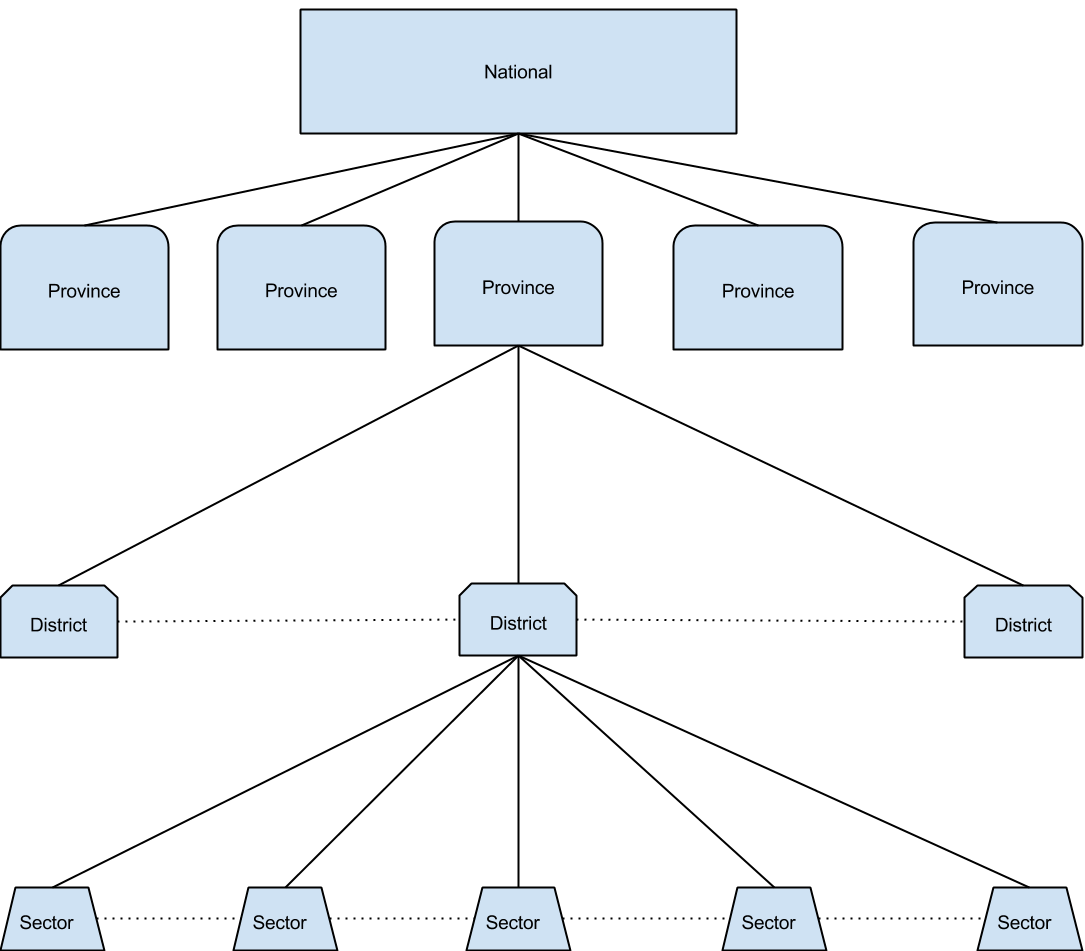
\includegraphics[width=12cm]{empirical/images/rwanda_administrative_division}
\caption{Rwanda Administrative Division}
\end{figure}
Because of its location it works perfect as a gateway to all countries in Africa. 
And due to the stable environment compared to many other contries in this part of the world, it is very attractive for foreigners to do business here. 
Making it the `Singapore of Africa'.

Rwanda has a goal of being transformed to a knowledge based economy with Information and Communication Technology or ICT. 
This means basicly that they want to offer ICT services for other kind of resources. 
They want to be the regional center for training top quality ICT\nomenclature{ICT}{Information and Communication Technology} professionals.
In turn, create wealth, jobs and entreprenaurs. 
From their perspective they have some competetive advantages in order to achieve this:
\begin{itemize}
\item Cheap labor compared to other countries in the Region
\item Young and dynamic workforce (98\% of the population is under 50 years and 43\% is under 16 years)
\item Most favorable business environment in the Region (8th best place to do business in the world 2012)
\item Low levels of corruption - Zero tolerance (Transparency international Bribery index 2012 ranked Rwanda as least bribery prone in the EAC)
\item World class ICT infrastructure
\item Strong \& visionary leadership
\item Bi-lingual business environment (French and English)
\end{itemize}
\cite{2}

\section{Brief History Lesson}
We start at the 14th centuary, when the Tutsies enters Rwanda. 
Before them there were two other peoples, Hutu, which means farmers and Twa who was the very first recorded prople in Rwanda.
There is some disagreement of what the differances are between the peoples, but origanily, Tutsies were cattle owners and the Hutus were farmers. 
About five hundred years later the first European visits Rwanda and in the same centuary Rwanda becomes a german protectorate. 
This makes Rwanda under the protection of Germany with some oblegations for their services.
Skipping fourth to 1933, now occupied by Belgian forces, all citizens are issued with an identity card defining their identity.
In 1962 Rwanda becomes independent and gets their 1st elected President. 
After this there is turbulent times for Rwanda. The Hutus and Tutsies are having violent reactions towards eachother with a peak in 1994.
A geneside primeraly by Hutu extremists, killed over 500,000 people, primeraly Tutsies, in the course of about 100 days. 
The genocide was triggered by the assasination of the Hutu president Habyarimana.  
The Tutsie Rwandian Patriotic Front, also known as the RPF\nomenclature{RPF}{Rwandian Patriotic Front}, takes action and took control of Rwanda the same year.
The current President, Paul Kagame, was a former member of the Rwandian Patriotic Front.
\cite{17}\cite{18}\cite{19}

\section{Information Technology focus in Rwanda}

\begin{figure}
\centering
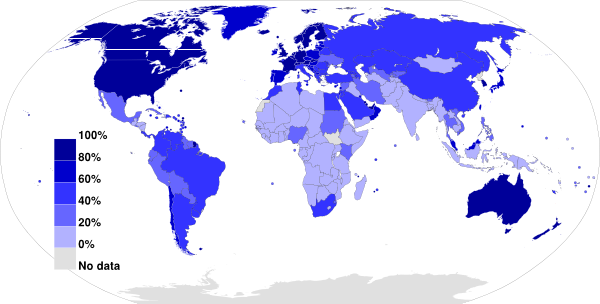
\includegraphics[width=12cm]{empirical/images/internet_penetration_2012}
\caption{Global Internet Penetration in 2012 \cite{3}}
\label{fig:global_internet_penetration_2012}
\end{figure}

\begin{figure}
\centering
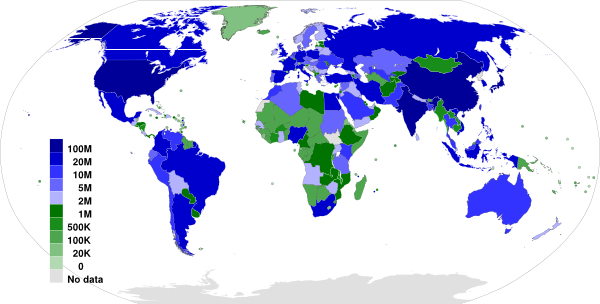
\includegraphics[width=12cm]{empirical/images/internet_users_2012}
\caption{Global Internet Users in 2012 \cite{3}}
\label{fig:global_internet_users_2012}
\end{figure}

Rwanda has an internet penetration of 7\% in 2012. 
In Africa there is an internet penetration of 15.6\% and for the world it is 34.3\% (See ~\ref{fig:global_internet_penetration_2012})\cite{4}. 
Rwanda had an increase of internet penetration from 1\% to 7\% from 2000 to the end of 2011\cite{2}.
More interesting is the mobile broadband development in Rwanda. 
The subscriber base accounts for 48.1\% of the population and the network coverage accounts for 99.79\% of the country.
Thus, the technology is there, but the hardware is not yet updated.
In general, people are using simple phones.
Some of these phones supports java and a very simple browser, but it cannot be compared to a working internet connection.
The government of Rwanda has made the decision to become an ICT hub in Africa.
Therefore alot of resources and attention is focused on developing knowledge in the field of ICT. 
As of january 2013 the Rwandian government is planning to set up an ICT park through the Rwanda Development Board.
This park will host technological training, industries research and development. The ICT park will support the growth of the following clusters:
\begin{itemize}
\item Energy
\item Internet, multimedia and mobile telecommunication
\item Knowledge
\item E-Government
\item Financial
\item ICT Service and export
\end{itemize}
\cite{2}
Also there were some rumors about free WiFi throughout all of Kigali.
They were in 2012 ranked among the top 6 developing countries when it comes to dynamic performance in ICT development\cite{5}.

\section{Health Information System Programme}
\subsection{About}
The Health Information Systems Programme (HISP) is a global network established, managed and coordinated by the Department of Informatics at the University of Oslo.
They design, implement and sustain Health Information Systems by a participatory approach\cite{8}. 
This means including the local users when develping the system in hopes of a more sustainable and successful project.
The system developed aims for supporting health care delivery and informaiton flows in selected health facilities, districts and provinces.
\begin{description}
\item[Vision] To strengthen the development and use of integrated health information systems within a public health inspired framework in India and the South Asian region\cite{9}.
\item[Mission] To enable networks of collaborative action with like-minded actors who aspire to the ideology of open source software, open standards and decentralized decision-making to create complementary strengths in providing integrated and public health friendly health information systems\cite{9}.
\subsection{History}
In the 1970 and 80's the HISP\nomenclature{HISP}{Health Information System Programme} approach to action research and system design was influenced by a number of union based action research projects in Scandinavia.
The focus were on empowering workers who were affected or threatened by new technology.
Methods may have changed over time, but the philosophy remains the same.
Explore ways in wich disadvantaged people could appropriate ICT's for their own empowerment.
Original key member of the HISP team had background as social political activists in the anti-apartheid struggle and other social movements.
DHIS\nomenclature{DHIS}{District Health Information System}, a software organized and developed within the HISP network, was actually born out of the political processes following the fall of apartheid\cite{7}. 
During apartheid and until 1994 there were 14 departments of health in South Africa.
Bacause of this fragmantation it was alot of different procedures, collection tools and data defenitions. 
In order to take this into account, DHIS became very flexible and one can easily see how this has effected the design. 
This might be the reason why DHIS framework could be used in other countries.

\subsection{District Health Information System}
\label{sec:dhis}
The latest version of DHIS during the case study was version 2.13.
DHIS2 is now used by over 30 countries across the globe and even more organizations.
DHIS2 is a tool for governments and health organizations to manage their operations more effectively, monitor processes and improve communication.
DHIS2 is mainly a tool for managing aggregate data. 
It will let you visualize large amounts of data in a GIS\nomenclature{GIS}{Graphical Information System} implementation, a pivot table and in charts. 
These data representations can then be shared with other user registred in the same DHIS2 instance.
Probably the most powerful feature would be GIS. 
This feature shows selected data on map based on province, district etc\nomenclature{etc}{Et cetera}. 
The regions on the map can then be colored based on the data. 
If one has data for the hole country one can in seconds get a accurate impression of the current health status. 
DHIS2 runs on server wich is connected to a database. 
As long as this server is connected, anyone with a decent browser and an internet connection could access and make use of DHIS2.
\subsubsection{GIS}
\begin{figure}
\centering
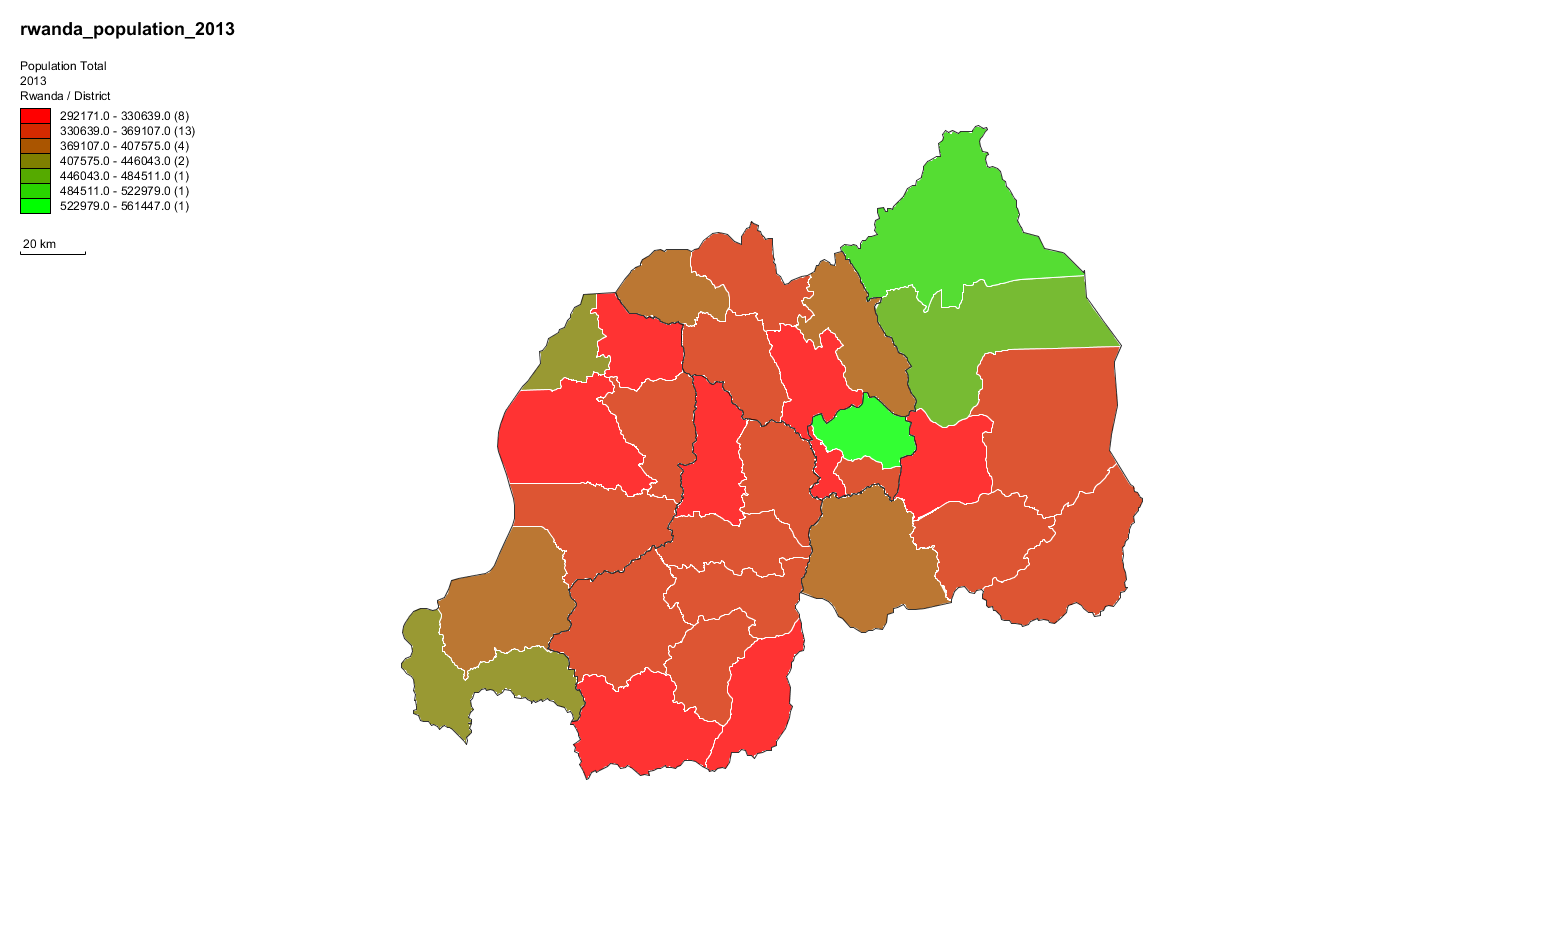
\includegraphics[width=12cm]{empirical/images/map_rwanda_population_2013}
\caption{A population count using GIS in DHIS2}
\label{fig:a_population_count_using_gis_in_dhis2}
\end{figure}
The GIS that is integrated in DHIS2 is relatively easy to use. 
One selects what kind of regions that are of interest and apply the correct data that should be visualized, see figure ~\ref{fig:a_population_count_using_gis_in_dhis2}.
Heres a list of some of the functionality that the GIS offers:
\begin{itemize}
\item Thematic mapping of areas and points.
\item Visualize catchment areas of facilities.
\item View facilites based on classifications.
\item Overlay multiple layers and use googlemaps as a background layer.
\end{itemize}\cite{10}
\subsubsection{Charts}
\begin{figure}
\centering
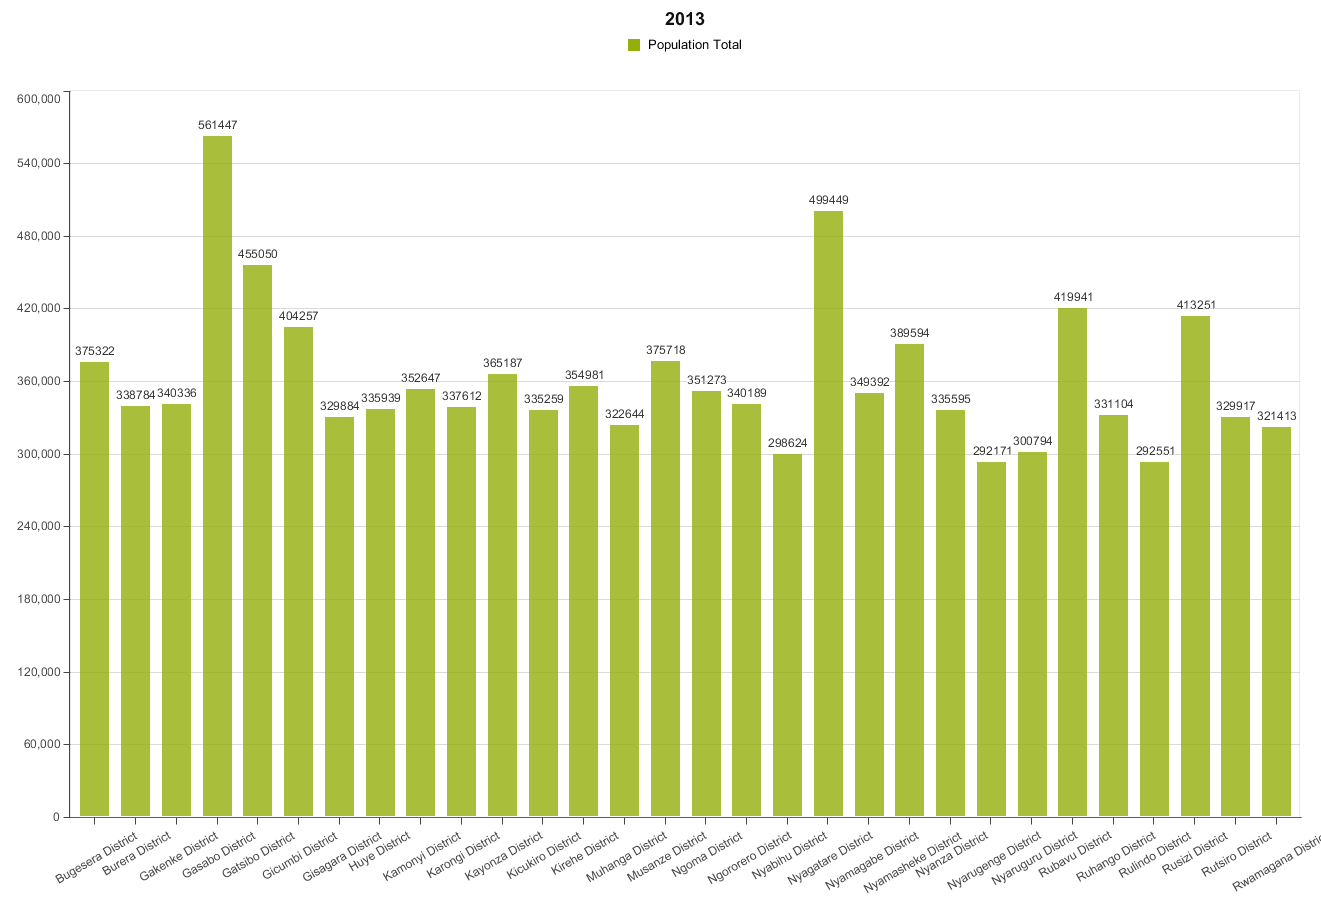
\includegraphics[width=12cm]{empirical/images/chart_rwanda_population_2013}
\caption{A population count using a chart in DHIS2}
\label{fig:a_population_count_using_a_chart_in_dhis2}
\end{figure}
The charts are a little bit trickier. In short the series is the y-axis and Category is the x-axis. Displaying data as a chart is allright once you get what the words mean.
Figure \ref{fig:a_population_count_using_a_chart_in_dhis2} shows an example counting population by district. Types of charts supported include:
\begin{itemize}
\item Column
\item Line
\item Pie
\item Stacked Column
\item Area
\end{itemize}
\cite{10}
\subsubsection{Pivot Table}
\begin{figure}
\centering
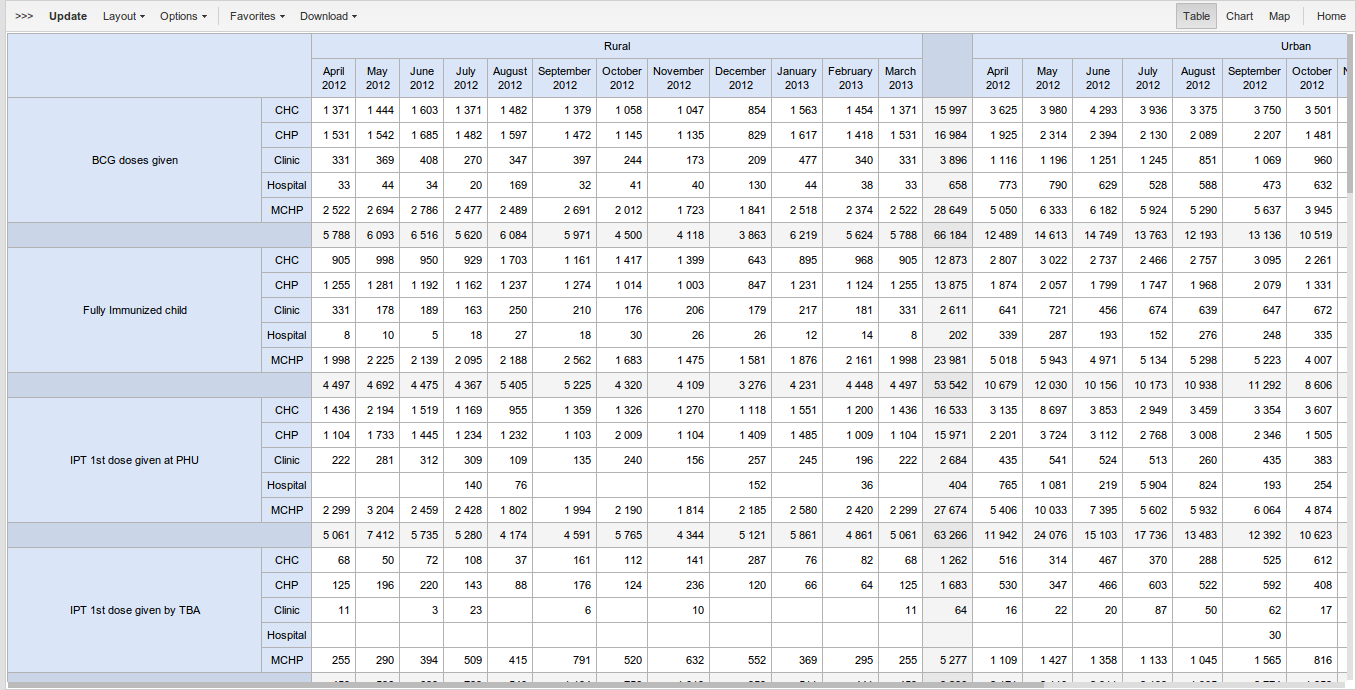
\includegraphics[width=12cm]{empirical/images/pivot_table_example}
\caption{An example of a pivot table in DHIS2\cite{10}}
\label{an_example_of_a_pivot_table_in_dhis2}
\end{figure}
A pivot table is a data summarization tool. It generally sorts data and show them in categorized table.
The DHIS2 pivot table let's you analyse data along all data dimensions and arrange these on columns, rows and filters, see \ref{an_example_of_a_pivot_table_in_dhis2}.
\subsubsection{Dashboard and social features}
One can send messages and share all data visualizations with users registrered on the DHIS2 instance. Interpretations of the visualizations can be commented and viewed by all other users. 
This way DHIS2 let's users experienced in the field help others interpretate the data while they are looking at it. Also one can store charts, maps and pivot table at a dashboard so they can easily be referenced later.
\subsubsection{Individual Records}
DHIS2 was mainly intended for aggregated data that could not related to anyone person. The need for a system which can track individuals is a requirement that most users of a health care system would want.
Therefore the DHIS2 tracker was developed. It let's you sign up people for programs and track them through the process. Also send out reminders so that patients come to their scheduled checkups. 
One problem with the individual records is that it does not work as a patient record system. Such a system is that it requires a level of confidenciality that DHIS2 currently is not supporting. 
Also a patient record system needs all health facillities to be users of the same system if it is going to be of any use.
\subsubsection{Data entry and validation}
DHIS2 let's users entry data even if their not online. 
This feature is crucial for countries with unreliable connection to the internet. 
For developing countries with regular power cuts, one can understand why this is. 
Data entry is done with prepared forms and then uploaded to the server which is running the DHIS2 instance.
The forms are highly customizable due to the varying requirements from users. 
Also there is the possibility to validate the input. For an example shouldn't there be more people under five years than people in the same region, just to give an example.
The data entry can be done in alot of different ways. 
One example is through SMS\nomenclature{SMS}{Simple Message Service}. In industy countries this may sound odd at first, but in developing countries health facilities might not have access to computers. 
This is the simplest form of data entry, even though it might require some coding of data representations. 
Since DHIS2 is accessible from any device with a browser the range of devices that can be used for data entry goes from a mobile phone that supports SMS to a sophisticated computer. 

\section{Healthcare}
The health care in Rwanda is still influenced by the genocide in 94, but compared to the state it was in back then, it's is in pretty good shape.
The health system is financed primarely the state, insurrance, individuals and direct fees for services.
The biggest health program is the Mutuelles De Sante. This is an insurrance based scheme.
Individuals pay a fee of 6\$ a year pr. family member and 10\% fo the service pr. visit.
The program started in 2004 and by 2010 91\% of the population had this insurrance policy.
Users of this system can go to a public and non-profit health centers, but are not allowed to use for profit health centers.
Although there's been alot of improvemnet in the recent years, the government still says that they have a long way to go to meet the countries needs.
\cite{20}
\subsection{History}
\subsection{Structure}
\subsection{Financial}
\subsection{Ranking and the rest of the world}
Two approaches. Participatory or export service.
\subsection{Health Information Systems in Rwanda}
The government instance that has the responsibility to maintain and manage health information data is the Ministy of Health. Here there is a team that maintains the Health Management Information System.
The HMIS \nomenclature{HMIS}{Health Management Information System} is built on open source District Health Informaiton System 2. 
The health ministry has made some modifications so that there is in fact 4 instances of DHIS2\nomenclature{DHIS2}{District Health Information System 2} running for different purposes.
\begin{figure}
\centering
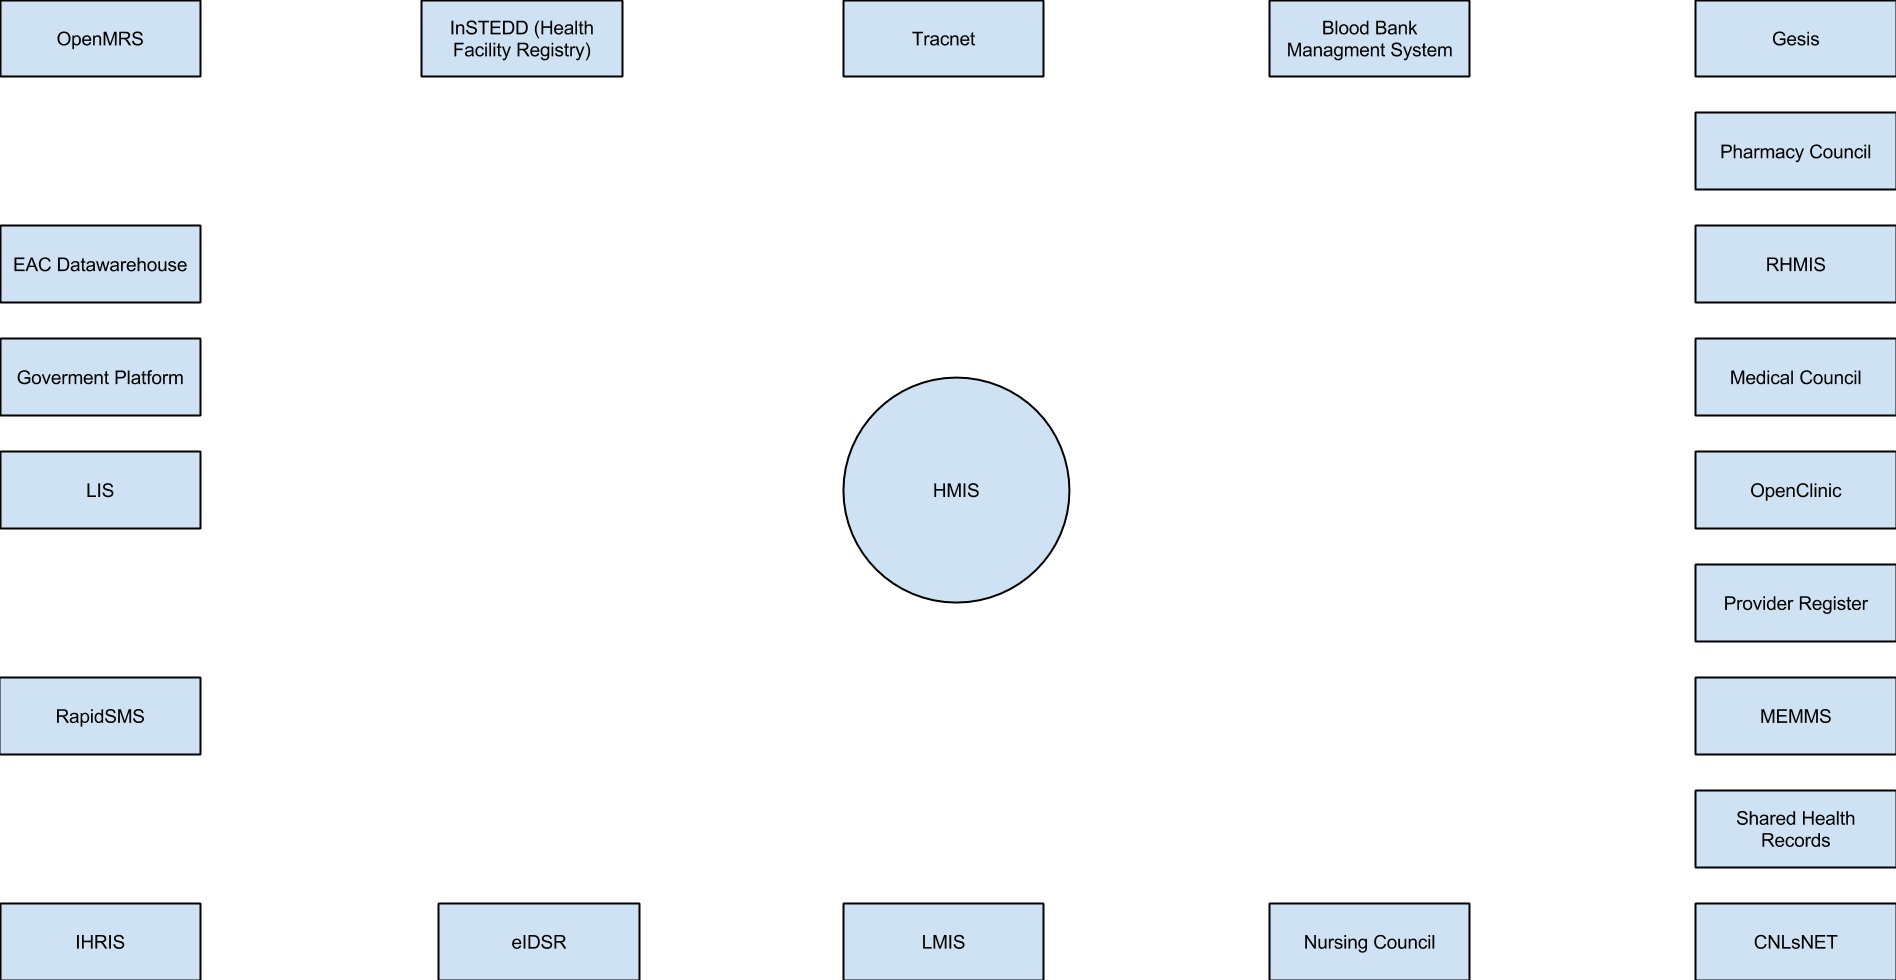
\includegraphics[width=12cm]{empirical/images/context.png}
\caption{Systems Currently in Use 2013}
\label{fig:systems_currently_in_use_2013}
\end{figure}
Besides the HMIS there are alot of systems that runs and has critical tasks that is not yet supported solely by DHIS2, see ~\ref{fig:systems_currently_in_use_2013}. These systems has varying tasks, but are all in some way related to HMIS.
Sharing data between these systems is crucial for maintaining an overview of the health status in all of Rwanda.
\subsection{DHIS2 enters Rwanda}





\chapter{Method}
\section{Shoice of Method}
\section{Data Collection}
\section{Reflection \& Data Analysis}
\subsection{7 Principles for Conduction and Evaluating}
\chapter{Case}


\section{Information Systems in Rwanda}
\subsection{Current situation}
The point of the whole study was to get an overview of the current situation and produce som kind of action plan from which we could set into action.
This case concerns Health Management Information System and their implementation of DHIS2. HMIS got the main responsibility to manintain and to facilitate the flow of health data from all of Rwanda. Even though they are the people with the main respnsibililty there are other actors as well. 
During the research period one of the main goals was to develop interoperability between the different actors concerning health information data. 
It is important to note that from this perspective, interoperability is seen through the lens how well other systems interact with HMIS and DHIS2.  
\subsection{Dataflow}
\begin{figure}
\centering
\includegraphics[width=12cm]{empirical/images/dataflow}
\label{dataflow}
\caption{Dataflow}
\end{figure}
In figure \ref{dataflow} you can see how the data flows from users all the way to the DHIS2 database. Actually the data from user all the way up to the health facilities is paper based.
These data flows would greatly benefit from transitioning to an electronic based system. The same is true for the district hospitals. Users usally collects data in a paper based version, but this is currently for conveniance. In the villages there simply isnt an alternative and data from villages is collected and aggregated at the health facilities. This causes a problem. Because all data is aggregated one cannot tell the differance between villages. Currently this is supported by the program offered by Voxivia. For an example, if a village would run out of some drug and another village in the same catchment area would have to much, the will report that the stock of drugs is good. The Voxivia on the other hand would report each village separately and therefore is still in use.
\subsection{Malaria Surveliance}
The malaria surveliance project consists of two main branches. 
\subsubsection{Sentinel Surveliance}
The malaria sentinel project is implemented and is currently reporting weather data and malaria cases, with some extra information.
The purpose of this instance is to map all malaria cases based on their geographical location and see if there is a connection with malaria data and weather data. 
It certainly is. 
\begin{figure}
\centering
\includegraphics[width=12cm]{empirical/images/sentinel_surveliance}
\label{sentinel_surveliance}
\caption{Sentinel Surveliance}
\end{figure}
The sentinels are differents stations spread throughout Rwanda. Adding up the sentinels catchment area they should cover all of Rwanda. 
Currently these stations data isnt integrated in DHIS2. This is a very simple task, but it needs to be coordinated by the leaders so that everybody is onboard with the solution.
DHIS2 is currently supporting all the requirements, but in order to make the transistion the personell doing the reporting has to be trained.
\subsubsection{Active Surveliance}
Active Surveliance is another branch of the malaria surveliance. The thing is, one wishes for data from the place were the malaria was first noticed.
This kind of data would include if the infected person has bednets, if others in the same house has malaria and other contextual data in hope of seing a pattern to what is most likely to make a person infected. Currently the health personell is using a paper based reporting form, but would like to transition to an electronic based report.
The technology that the health workers currently are equipped with is usally regular simple phones that could interact with DHIS2 with SMS. DHIS2 is supposed to support this feature, but it is not been properly tested. A requirement is that one would have to set up a SMPP\nomenclature{SMPP}{Simple Message Pear-to-Pear} gateway with a local teleoperator. In this case the most likely would be MTN.
The technical expertise for this kind of functionality isnt the main obstacle. It's the bearucracy. The decicion process is long and it takes a while just to map who to talk to about what before one could even start testing.
\subsection{External Systems and DHIX}
\begin{figure}
\centering
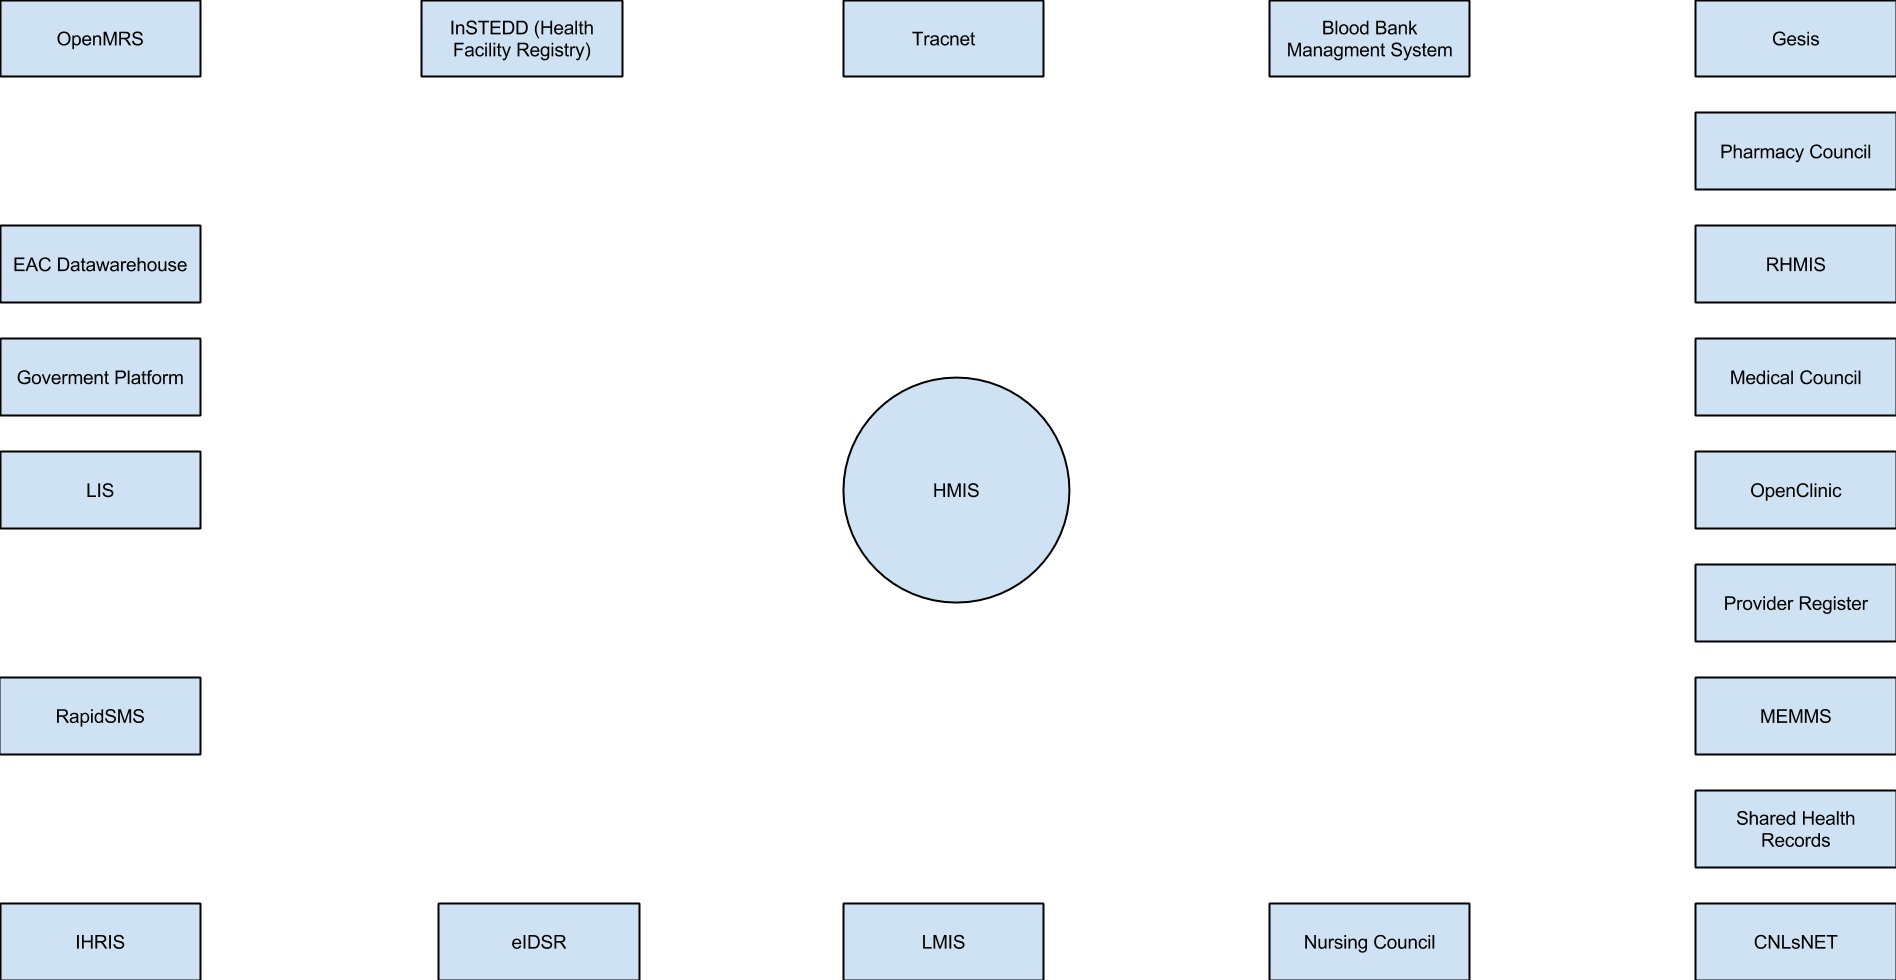
\includegraphics[width=12cm]{empirical/images/context}
\label{external_systems}
\caption{External Systems}
\end{figure}
Figure \ref{external_systems} shows the systems that got mapped during the case study. DHIX represents the HMIS system. The HMIS is currently running four instances of DHIS2 with some scripts for synchronizing data between instances.
\begin{figure}
\centering
\includegraphics[width=12cm]{empirical/images/future_design_rwanda}
\label{future_design}
\caption{Future Design}
\end{figure}
The HMIS has a vision on how they would like to interact with other systems, see \ref{future_design}. HMIS would like to collect all Ministry of Health systems under one roof. Then they would like to make some kind of interface between health ministry and other ministry systems. The specifics of how this is going to work are not decided yet. The ministry of health would like to be able to exchange data with external systems as well. This is done via an access layer. Between this access layer one would be able to synchronize data with external systems. For instance, there is a system called Voxivia that has data that is more specific than what is currently supported by the DHIS2. These data would be of great benefit to the HMIS. 
\subsubsection{DHIX}
DHIX is the name that we gave the system at the HMIS. As mentioned, this system consists of several subsystems.
\begin{description}
\item[HMIS]General health statistics for Rwanda. 
\item[Health Finance]Contains data for performed health services. Like a treatment program. This data is used for Performance Based Finance, \nomenclature{PBF}{Performance Based Finance}PBF. PBF allocates resources based on how well the facility is performing.
\item[Individual Records]Contains data specific to individuals using the tracker module in DHIS2.
\item[Datawarehouse]This instance has all the important statistics of the other DHIS2 instances.
\end{description}
\begin{figure}
\centering
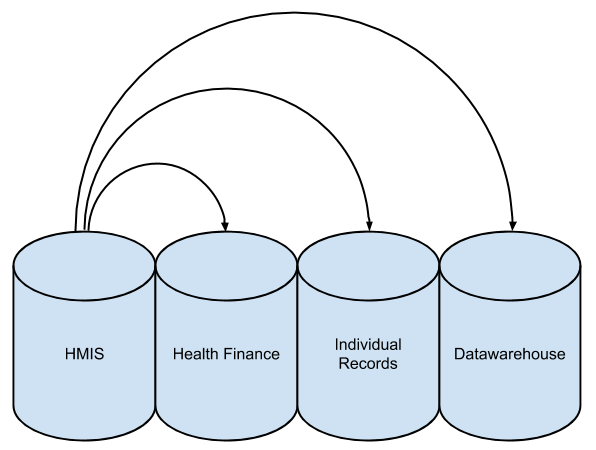
\includegraphics[width=12cm]{empirical/images/hfr_dhix}
\label{hfr_dhix}
\caption{Health Facility Registration in DHIX}
\end{figure}
When it comes to Health Facilities the different systems has to synchronize with eachother. As in figure \ref{hfr_dhix}, the HMIS server should be able to push data to the other instances of DHIS2. In the future, the HMIS would like to make it possible to push data groups into other instances of DHIS2 as well as health facilities.
\subsubsection{Health Facility Registry}
Currently the registration of new health facilities is done on a platform developed by inSTEDD, also known as the HFR\nomenclature{HFR}{Health Facility Registry}. The HMIS is planning to do this registration at the HMIS instance of DHIS2. The inSTEDD platform is used by all external systems that uses the list of Health Facilities, so in order to transition this functionality to DHIS2 all systems that  depends on this service has to be on board. 

\part{Discussion}
\chapter{Conclusion}
\begin{thebibliography}{99}
\bibitem{1}http://en.wikipedia.org/wiki/Rwanda , {\bfseries 2013}, {\itshape Wikipedia}
\bibitem{2}http://www.rdb.rw/rdb/ict.html, {\bfseries 2013}, {\itshape Rwanda Development Board}
\bibitem{3}Percentage of Individuals using the Internet 2000-2012,{\bfseries 2013}, {\itshape International Telecommunications Union (Geneva)}
\bibitem{4}http://www.internetworldstats.com/stats.htm, {\bfseries 2013}, {\itshape Internet World Stats}
\bibitem{5}http://www.newtimes.co.rw/news/index.php?a=62858\&i=15239, {\bfseries 2013}, {\itshape Kigali Trade Zone to host ICT park}
\bibitem{6}Luis Guijarro, {\bfseries 2006}, {\itshape Interoperability frameworks and enterprise architectures in e-government initiatives in Europe and the United States}
\bibitem{7}Jørn Braa and Sundeep Sahay, http://www.mn.uio.no/ifi/english/research/networks/hisp/hisp-history.html, {\bfseries 2013}, {\itshape The Process of Developing the DHIS}
\bibitem{8}http://www.mn.uio.no/ifi/english/research/networks/hisp/index.html, {\bfseries 2013}, {\itshape HISP}
\bibitem{9}http://hispindia.org/index.php/about-us, {\bfseries 2013}, {\itshape About HISP}
\bibitem{10}http://www.dhis2.org/data-management, {\bfseries 2013}, {\itshape Data management and analytics}
\end{thebibliography}
\appendix
\chapter{Journal}
\section{Day 1}
\begin{tabular}{|c|c|}
\hline
Date: & 07.10.2013 \\
\hline
\end{tabular}
\subsection{Traveling}
\subsubsection{Bus}
I started out with waking up at 05:00am. Usually I get my salary from Peppes at the 7th each month, but this time there was a delay.
So waking up, I was broke. No money for the Planebus. I tried to get some money from the local gas station with my mastercard with no luck.
With only 3minutes until my bus was leaving i hoped that the bus driver would accept my mastercard. He did.
Either way i was in luck, just before I was going to pay i checked my balance and my salary was in.
\subsubsection{Trondheim Airport}
No problem here. Talked a little with my mom, said goodbye and registrered. Plane ride was good.
\subsubsection{Oslo Airport}
Met up with Simen. There was some problems with he's visa. One cannot leave Norway and have a visa that expires before your return date.
He had fortunately bought a flex ticket so he could just change the dates, and then change them back when he arrives Kigali and prolonges his visa.
Then it was off to Istanbul. Flight was ok, good movies.
\subsubsection{Istanbul}
A little short on time. Didn't find the directions to our gate at first. The signs were properly hidden. After a little exploring we found it. Next stop, Kigali.
The flight seemed a little longer, but it was cured by `free cell' and `soduko'.
\subsubsection{Kigali}
At last, after about 18 hours from Trondheim, I was here. The guy that checked out our visa seemed a little sceptical, asked me one more time of my purpose of visit.
I just explained that we had an internship with the Management Sciences for Health and it was ok.
Felix picked us up and drove us to our house, 21KK Avenue, Niboye Road.
Awsome house! Randy's old place. We could stay here for free out October.
Took a beer with Felix and went to bed.

\section{Day 2}
\begin{tabular}{|c|c|}
\hline
Date: & 08.10.2013 \\
\hline
\end{tabular}
\subsection{Meeting with Randy}
\subsubsection{Breakfast}
Got off to a bad start today. Woke up 10:05AM and we were expecting Randy at 10:00AM. No worries though, he wasn't there yet.
Took a shower. Simen sat outside talking to our day-time guard, Peter.
I took some breakfast, bread with jelly, a tomato and a banana. The bananas here are very small. Anyways, Randy came in the middle of breakfast and we talked some.
\subsubsection{Bank}
Then we drove out to the bank. About a 5 minute drive I think. We took out 100 000RFR, this should cover us for about 2 weeks Randy said. About 1000NOK.
Then we had to get our SIM-cards.
\subsubsection{MTN}
Pretty straight forward. We registreded our passports and got our sim cards with unlimitided data usage.
\subsubsection{Lunch}
We got liuch at a chiniese resturant. The food was not very great, but better than airplane food I think. Strong chilli. We got chicken, goat and some vegetables.
Simen and Randy were so kind and decided that for me.... 
We then got to talk about the project. In general I think we got 3 options.
Malarya registration by phone, system migration from Voxivia and a bigger project that involved several Systems and a Data warehouse.
The systems included HMS, Inidcator Remarks and health finances. The data warehouse should also be able to pull data from several instances.
We did not land on a specific one and we were presented with some other options as well.
The project that involved several instances had alot of subproject bound to it.
Andrew is the system wizard, Eric the doctor that likes his ways and Beth is a eager IT-person.
Randy talked a little about another survey that he thought was better than DHIS2. We should gather some recomendations here I think.
\subsubsection{The Office}
Then we went down to the office were we will probably work. Our space consists of 4 cubicals that we share with 2 others.
It was not far from the ministry of health.
\subsubsection{Back Home}
Randy had to go to a meeting so we called it a day. We were invited to join a training program on thursday later this week. Meeting up with Randy 08:30AM tomorrow.

\section{Day 3}
\begin{tabular}{|c|c|}
\hline
Date: & 09.10.2013 \\
\hline
\end{tabular}
\subsection{First day at the office}
We were drown from our house to the ministry of health by Randy today. 08:30AM. Early day. Randy had some meetings and we've got the oppertunity to chack our emails and catch up on some reading. I found some new articles today that talked a little about how there is a gap between some countries in the IT world. Talked a little with Simen about ttrying to share our perspectives to get the best from both worlds.
\subsection{DHIS2 Intro}
After a while Randy was finished with his meetings. Andrew, the system wizard, came and said hello. He is joining us tomorrow for some DHIS2 training.
We where introduced to alot this session. Mostly about how they were using DHIS2 today. DHIS2 is not the only program they use. The functionality that are needed, but not supported by DHIS2, are hacked into their day-to-day work with some scripts made up by different people. I think their data is pushed to the server monthly. \\
Here is some changes that Randy suggested.
\begin{itemize}
\item Wanted to make some good validation rules, but lacked people with experience in the field to make them proparly.
\item After the usercount got high, the favorites got very messy and unorganized.
\item Would like to share tables, diagrammes and maps with individuals and make only a selected few public.
\item Some labels on the map, didnt quite get that one.
\item They would like to choose what type of faccilities that would be viewed in GIS. This would be a great improvement.
\item They had some language barriers. Would like som improbements there. Didnt get the details.
\item Problem with reports being loaded from NGINX cache, they were not updated after changes if it already was in NGINX cache.
\end{itemize} 
I was wondering how he trusted the data. It turned out that sometimes the data wasnt accurate. This was tested by some people motivated by a Performance Based Finance system. The health facilities down here get some funding based on their registration count. Some cases are worth more than others. Like, dont actually know the numbers, but lets say 1000RWF for registrating a pregnant woman. So to prevent health facilities from cheating the authoreties take some samples in order to check if the inputed data is correct. Randy would like some more competance on iReport. Should check that out later. FOSAID is the identification number used through all the databases. This identifies the facility. This number is also used by external systems. I think I should get a better understanding of Pivot tables. They are quite popular here. Camel is used to make an access level from the MOH to extarnal systems.\\
He also gave us an overview of how everything should be linked together in the future.\\
\includegraphics[width=15cm]{appendix/images/future_design_rwanda}\\
I then wondered how they could trust the open source code to do its job. Is there some testing that ensures that DHIS2 is working as it should? To me this seems like life or death for some people. When funding is based on registration of data. Is this the only option that MSH have? What other options did they consider before DHIS2? And what was the primary factor for choosing DHIS2. Open source? Proprietary softerware alternatives? I know I would be very sceptical to a software that did not guarantee customer support. 
\subsection{Lunch}
During luch we got some food from a burger diner. Good food, bad smell around the toilet. Randy just had a baby that is 4 months old with his second wife from Rwanda. She had family in Trondheim and visited them not to long ago. 
\subsection{Install Rwanda DHIS2}
When we got back we installed all the necesarry software. We got our own copy of the database so that we could work localy on our machines.
\begin{enumerate}
\item JDK
\item Postgres
\item Ireport
\item Tomcat
\item odbc
\item restore database
\item edit hibernate.properties
\end{enumerate}
I think I should get more comfortable with enviroment variables in Windows. 
I should get back to my todo list for sure.
\subsection{Dinner}
After work we ate at a Italian resturant. A little bit pricy. Should probably find some cheaper alternatives.
We are getting picked up at 07:30AM tomorrow, so I should probably get some sleep now. Good NIGHT!


\section{Day 4}
\begin{tabular}{|c|c|}
Date: & 10.10.1987 \\
\end{tabular}
\subsection{1st session: Review of training}
The datamanagers from different facilities reviewed their previos training. See email from Gloria for more information.
Wheres the map? (Because they removed it.)\\
Inser chart list maybe to long.\\
Why is the top border gone in gis? (Problem solved)\\
Wheres the back button? (Found it!)\\
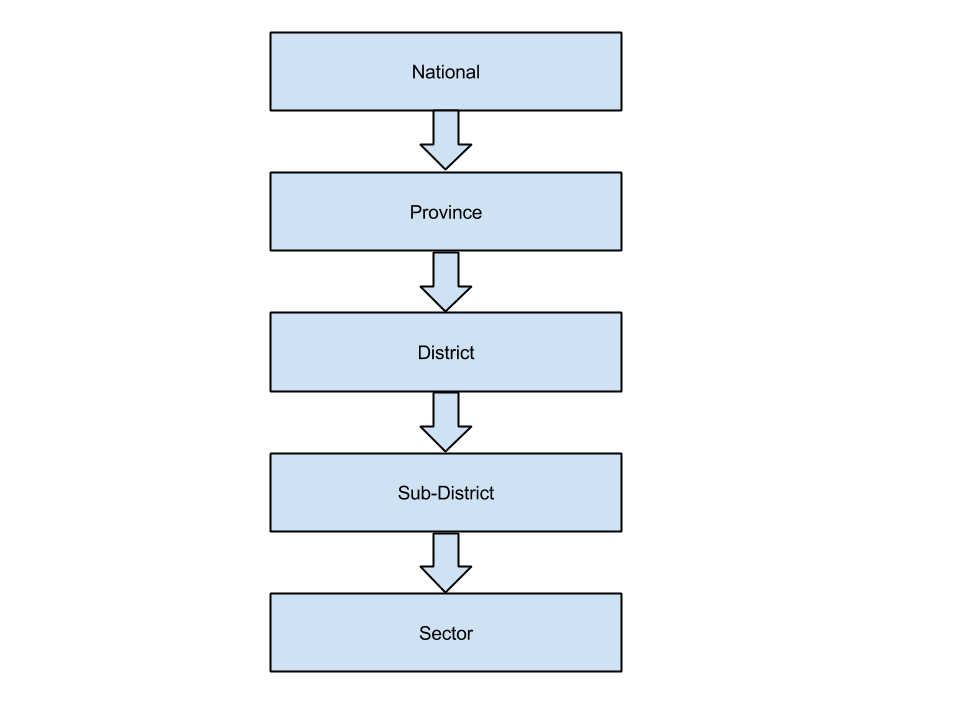
\includegraphics[width=15cm]{appendix/images/dhis2_map_categories}
\subsection{Meeting}
We talked a little bit here in order to get a better understanding of how they used the DHIS2. The consisted of me, Simen, Gloria, Adolf and three other data managers. It was a little difficult at first, but after a while I think we've got a pretty good understanding of it. They use DHIS2 for data analyses and for reporting data. Reporting data is done by the data manager at each health facility. Data analysing is used by monitoring and evaluation officer and head of community officers for decision making and strategic planning. \\
\includegraphics[width=15cm]{appendix/images/Dataflow} \\
The collecting of data starts in paper form. They are then gathered at each facility for reporting in the DHIS2 database. They have a seperate reporting system with voxivia. They still use this because they allow for more detailed information. If they use DHIS2 they have to track the reporting to the paperbased forms in order to get the ground details. Adolf mentioned that he would like a way to combine the data from the tracker and the aggregated data. This was a nice feature that they would like.
\subsection{Dinner}
Dinner was awsome!
\subsection{Second Session}
We then had a look at their presentations. We only stayed for one presentation. Then it was photo's. Thumbs up Simen!

\section{Day 5}
\begin{tabular}{|c|c|}
\hline
Date: & 11.10.2013 \\
\hline
\end{tabular}
\subsection{MSC Office}
We set up at the Management Sciences of Health office. We met alot of new people. Mircel, I don't really know what he does yet. Think it was finance. Felix, good to meet him again. Bob the american. Cedrick and Emmir. Cedrick is a little shorter than Emir. And some other people.\\
\begin{figure}[p]
\centering
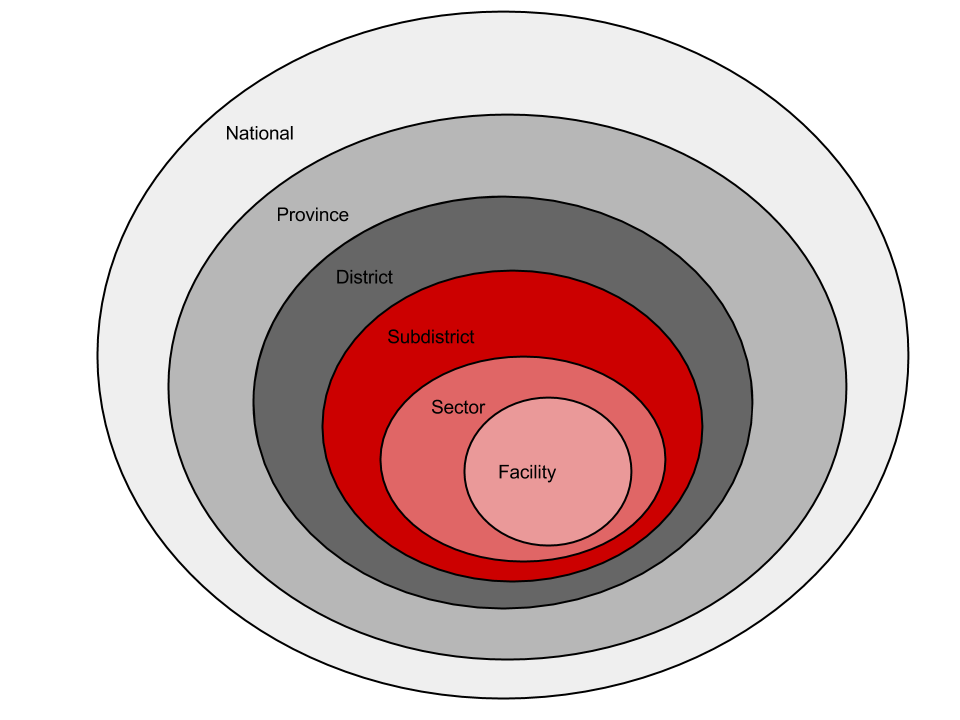
\includegraphics[width=15cm]{appendix/images/dhis2_rwanda_map_hierarchy}\\
\caption{Rwanda Map Hierarchy in DHIS2}
\label{Rwanda Map Hierarchy in DHIS2}
\end{figure}
\subsection{After Brunch}
After Randy's meeting we talked a little more about the projects that are relevant. The malaria surveliance and the interoperateabillity. I want the Malaria Surveliance. This would give us a concret assignment and a `know when its done' thing. The interoperateability would probably give us the best learning experience. Because it challenges me to think at computer systems at a higher level. I will send an email to Eric and discuss it further. I have a feeling I wont enjoy the best choice. Nappolina is the project manager.
\subsection{Conference room}
Randy gave us a briefing about the 2 remaining projects. This was alot of information to take in. 
\subsubsection{Malaria Active Surveliance}
The want to copy an existing report to a web based solution. Where this should be, I do not know.
\begin{itemize}
\item HTML
\item DHIS2
\item Mobile SMS
\item App
\end{itemize}
This was an extensive report. Randy proposed that we should mayby trim down the report a little. I think we've got the report on an email.
\subsubsection{Sentinal Surveliance}
This system is awsome. It's purpose is to collect weather and malaria data in order to see if theres an corelation between the two. They are going from 11 to 16 sentinels nationally. 
\begin{figure}[p]
\centering
\includegraphics[width=15cm]{appendix/images/sentinel_surveliance}
\caption{Sentinel Surveliance}
\label{Sentinel Surveliance}
\end{figure}
\subsubsection{Ineroperateability}
Then got of to discuss the interoperateability project.
For starters Randy wanted to make a report based on some choosen indicators.
The task goes something like this.
\begin{enumerate}
\item Load data from dictionary
\item Choose indicators
\item Choose metadata/attributes
\item Produce report (Maybe with a preferred layout)
\end{enumerate}
He then explained how he wanted the entire system to work.
The result would be something like this.
\begin{figure}{p}
\centering
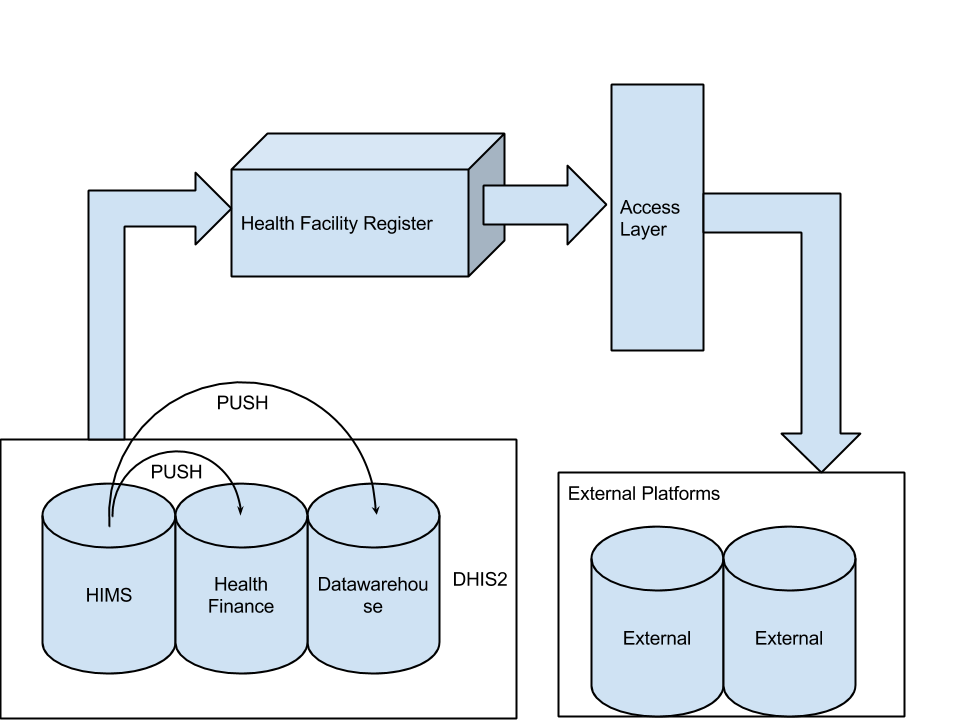
\includegraphics[width=15cm]{appendix/images/System_Architecture}
\caption{System Architecture}
\label{System Architecture}
\end{figure}
I think I should reaad up on SQL. It seem that this would be relevant.
For the last part he talked about how he would like to synchronize changes made to certain data element groups, cross instances of DHIS2. This in the case of adding adding elements. Would he like the same thin for indicators, I do not know. 
\subsection{Dinner at Randy's}



\section{Day 6}
\begin{tabular}{|c|c|}
\hline
Date: & 12.10.2013 \\
\hline
\end{tabular}
\subsection{HASH}
\subsection{Papairus}


\section{Day 7}
\begin{tabular}{|c|c|}
\hline
Date: & 13.10.2013 \\
\hline
\end{tabular}
\subsection{Spaghetti Dinner}


\section{Day 8}
\begin{tabular}{|c|c|}
\hline
Date: & 14.10.2013 \\
\hline
\end{tabular}
\subsection{Zero Values}
Today we got working on fixing  a database that had accedently deleted some 0's. Randy want to delete all zeroes from a specific date and then insert the ones from the last week or so. I thought this should be done directly with the database. This worked fine, but resulted in dates being placed instead of a NULL. I think this is very wrong. Should probably mention that we had a problem with the dataset. The booleans and the dates where not always present. This caused POSTGRESQL to stop when we tried to import the data. So Randy filled in all the empty values. This resulted in the same way as the other way.


\section{Day 9}
\begin{tabular}{|c|c|}
\hline
Date: & 15.10.2013 \\
\hline
\end{tabular}
\subsection{Before lunch}
We've just had a solution. We first import the data that should be updated. Then we import data with the right zeros. We then select the records that should be updated and do so. NP I think..... I think the only troubling part is learning how to use SQL and the operating system. On thing should be mentioned before I forget. There is some efficency issues I think. I do think that it would be better if they learn a little more LINUX since they have the server.
\subsection{After lunch}
We have a solution for the database problem. We need to test it in order to be sure. Bah, lot of work. Anyways, this is important. So, moving on. We think we could implement the data entry report in DHIS2. This is fairly easy. We found a bug in the program. After creating the data elements and indicators and adding them to a dataset. We then bound them to an organisation unit, but the set would not show up. After deleting the set and re-insert them, DHIS2 would suddenly find them. Kinda important I think. That's about it.
\subsection{House hunting}
We've went to a couple of places for Simen's last days. I should probably look for a hotel or so for the last days here. I will tallk with Randy tomorrow. Scary shit the last place we were at. Simen did not think so much about it. The first place we went to was great though. Awsome, I would prefer to live there when I come back again after Christmas.


\section{Day 10}
\begin{tabular}{|c|c|}
\hline
Date: & 16.10.2013 \\
\hline
\end{tabular}
\subsection{Staff meeting}
We had a staff meeting today. Topics of the day was.
\begin{enumerate}
\item HMIS portal. Andrew got assigned to this. I really don't know what kind of portal this is. Maybe a website for the public?
\item Clean up DHIS2. Since everybody had recieved training in how to use the DHIS2 there been alot of analytics that has been made. This resulted in making browsing very unorganized. Gloria got the assignment of cleaning this up and making a naming convention.
\item New systems to the DHIS2.
	\begin{itemize}
	\item TRACNET. Dont know its purpose yet.
	\item CNLS. Dont know its purpose yet.
	\end{itemize}
\item Annual report. I was wondering what this report should contain. Are they using DHIS2 in order to make this?
\item NIKE foundation. I didn't mention this, but I think there should be some research about what they are doing since the guy at the `good house' was saying that they were doing alot of similiar things. My first idea was that we should share databases. But who knows, maybe there is some competition going on here.
\item SMS module. I really didn't get what this was really about. There is an easy way to do the dataentry in DHIS2, but there were some interest in the group of having an alert system based on some thresholds. I was thinking this should be done with an app.
\item DQA. This is an abbrevation for Data Quality Assesment. The main problem was that they would like to compare their data with samples from the field. DHIS2 does not support this functionality very well. This is a possible task. Something was mentioned about a report card that is being developed or been developed, but I didn't quite follow.
\item Then it was the Resource mapper. This relates to the overall architecture and the interoperateability thing. Gloria, Randy and Bob are working on this. 
\item The group is planning a training early this November. Should be thinking about growing a mustache. Anyways, the group is going to be trained in iReport and HTML report. Randy is putting this together.
\item We should upload some database files to the Gorilla server. Gesis HC and Gesis DH. Eventually putting them in the DatawareHouse.
\item At the end of the meeting it was mentioned that some of the members should think about their contracts. Are they looking for other jobs? Got me thinking about if they had secure jobs. What is their situation there?
\end{enumerate}


\section{Day 11}
\begin{tabular}{|c|c|}
\hline
Date: & 17.10.1987 \\
\hline
\end{tabular}
\subsection{Setting up for Development}
There's a slow internet connection here. This is something thats significantly slows down the process in generel. I download in general about 50kB/s tops. Upload seems to be the same. The eclipse set-up seem to work fine. Got some errors with the maven plugin for eclipse. So I decided to run maven outside eclipse and then import it in. We use bazar as version control. I had a unicode problem when trying to push our branch to the server.
\subsection{Meeting with Edith}
Time: 02:00PM, I got a meeting with Edith later to discuss setting up an SMPP account with MTN (the local teleoperator). Hopefully will get to the bottom of this. A previous master student, `Magnus', tried to set this up, but he was met with indecision I think. We agreed that Edith should make arrangements for a SMPP Gateway. How i'm really not sure. Hope that it will get done.


\section{Day 12}
\begin{tabular}{|c|c|}
\hline
Date: & 18.10.2013 \\
\hline
\end{tabular}
\subsection{Continuing setting up IDE}
We will use Eclipse. Everyting should be ready. I encountered a problem building the project with Maven. There were some test's that would produce some errors.
When we skipped the test's, everything seems to work. We agreed with Randy that we will work on Interoperateability. Also agreed with Eric that this is what we shall be working on. Hopefully we'll starrt on monday.


\section{Day 13}
\begin{tabular}{|c|c|}
\hline
Date: & 19.10.2013 \\
\hline
\end{tabular}
\subsection{House hunt finished}
Simen decided to move in the house next to the MTN center.
\subsection{2nd Hash}


\section{Day 14}
\begin{tabular}{|c|c|}
\hline
Date: & 20.10.2013 \\
\hline
\end{tabular}
\subsection{Showing Felix the House}
This day we showed Felix where Simen will live for the remaining 2 months.
Felix had also made arrangements for me to live at a hotell for the last 2 days.
\subsection{Massage}
\subsection{Eating}
Biggest meal I've ever had. 

\section{Day 15}
\begin{tabular}{|c|c|}
\hline
Date: & 21.10.2013 \\
\hline
\end{tabular}
\subsection{Getting in touch with the Health Facility Registry}
Gloria is going to send me an email about this system. We will try to make the interoperateability thing work.
As of now we got many things going on at the same time. Honestly I don't know what we should be working on.
\begin{enumerate}
\item Interoperateability project.
	\begin{enumerate}
		\item Get current status from Bob.
		\item How often should the HMIS database update HFR?
		\item The data that should update HFR.
			\begin{enumerate}
				\item Where are they?
			\end{enumerate}
	\end{enumerate}
\item Malaria Active Surveliance.
	\begin{enumerate}
		\item Implement SMS gateway.
		\item Find out what happend to the Sentinel Project.
	\end{enumerate}
\item Import additional datasets and plan launch of National Data Warehouse and web portal.
	\begin{enumerate}
		\item Don't really know what this is..
	\end{enumerate}
\end{enumerate}

\section{Day 16}
\begin{tabular}{|c|c|}
\hline
Date: & 22.10.2013 \\
\hline
\end{tabular}
\subsection{Back at the office}
Got really sick yesterday. I think it was food poisioning. Now I'm back almost well again.
I hope that we can focus on the interoperateability project from now on. 
Simen suggested that we should make some interviews and I think that is a good idea.
We are going to get a breifing from Randy 10:30AM.
\subsection{Meeting with Randy}
We discussed the core issues of trying to synchronize their data. First of all it should be mentioned that the main issue here is to understand the problem. The problem being that they want to sync datavalues. The rest is for the moment irelevant. Datavalues is found in a table in the database. The table itself is called datavalue. Each record is identified by a primary key. In this instance this is a combination of id's. 
\begin{enumerate}
	\item dataelementid
	\item periodid
	\item sourceid
	\item categoryoptioncomboid
\end{enumerate}
The problem here is that these identifiers will not be the same in other instances of DHIS2. So in order to copy this data from one database to another we will have to find a way to compare the datavalues and decide if two values are the same or not.So actally there might be a datavalue that is the same, but with different identifiers. For the dataelementid there is a code that we could use that will be the same in all instances, but is this only for DHIS2 here in Rwanda? For the periodid we will have to compare start dates and period type.
The sourceid is the organizationunit. There is a code here that I hope is the same as the FOSA ID. 
And what exactly is the categoryoptioncomboid? In any case we should be able to make codes for all the categoryoptioncombos as well.  
\subsection{After lunch}
Should really find some proper food down here. The trick now is to make all the necesarry codes. These codes have to be the same for all instances of DHIS2. How are we going to facilitate this? The thing that is causing all the complexity is that they want independent databases. These databases don't sync completely. I don't know why they want it this way.
Thing is, how is access to all data a bad thing? Are there some security issues here? Randy told me that the different departments dont want other departments changing their data. So it's about wanting control of their own data I think. More openess could cause a drop in the data quality.
Delay...delay...delay.
Simen suggested that this would be a good thing in a different case. The regional database need data from only a selected data elements. This is in fact the same problem we're dealing with here.
Another issue that comes to mind is testing! We will have to make tests that ensures our solution.

\section{Day 17}
\begin{tabular}{|c|c|}
\hline
Date: & 23.10.2013 \\
\hline
\end{tabular}
\subsection{Starting on the interoperate ability project}
We discussed what the requirements for our case should be.
Randy wants to be able to transfer data groups from one DHIS2 instance to another.
We started to make some ideas and landed on making a web app. There were several good options.
\subsubsection{Android App}
This one we disqulified pretty early on. I think it was because it is kind of separate from DHIS2.
\subsubsection{Web App}
We thought this would be a good idea. This can easaly be integreted later on as a DHIS2 app and then run as a part of DHIS2.
\subsubsection{DHIS2 App}
The app framework is was not great for our purposes so we could not use it yet.

\section{Day 18}
\begin{tabular}{|c|c|}
\hline
Date: & 24.10.2013 \\
\hline
\end{tabular}
\subsection{Presented our idea to Randy}
Our idea was to make a webapp that will cover Randys requirements.\\
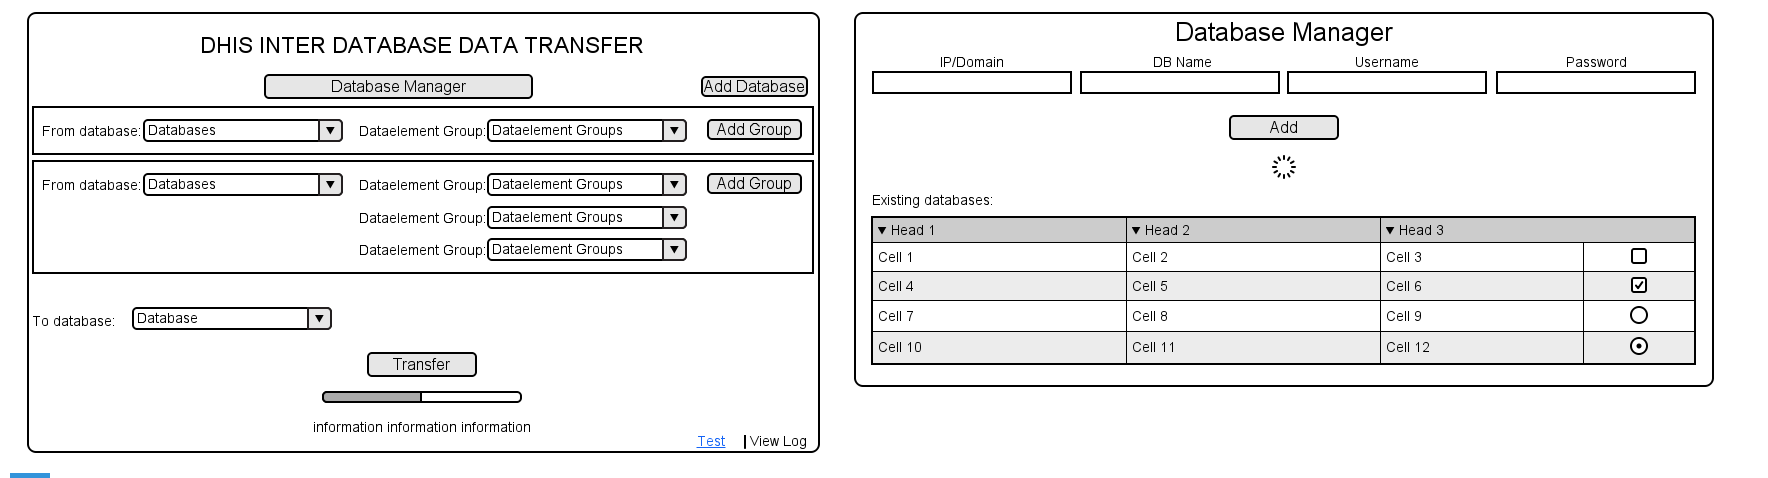
\includegraphics[width="15cm"]{appendix/images/mockup}
I started programming the GUI while Simen took care of the database.
Here the complications startet. We need a way to push datagroups into the other DHIS2 instance.
The web API does not support this.
So in order to do this we have to directly access the database. 
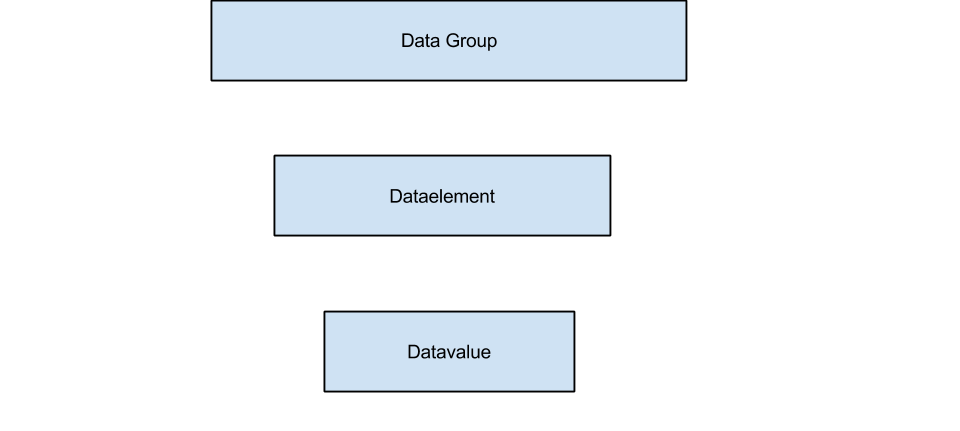
\includegraphics[width="15cm"]{appendix/images/datagroup}
The datagroup consists of several dataelements and a dataelement consists of a datavalue in DHIS2.
In the database it is a different story. There are alot of dependencies. So just pushing everything in would not work.
A problem is that groups, dataelements and datavalues may be there already. Also there is no way that the data is from one DHIS2 instance can identify the same data in another DHIS2 instance. We then thought of a way to handle this. 
Make codes that are equal cross instances and this way make comparison possible.
Dependencies in the database made this not so straight forward. There is a lot of dependencies in the target database that needs to be updateted when introducing new dataelements. I think this was solvable with a recursive algorithm. Simen did not like this. It seems that poking around in a database is not very popular. 

\section{Day 19}
\begin{tabular}{|c|c|}
\hline
Date: & 25.10.2013 \\
\hline
\end{tabular}
\subsection{Starting today's work}
Today we had a heated discussion regarding how to proceed. I still think that we should proceed, but in a slightly different manner. Simen think that users should be able to make the dataelements manually. I think it should be automated. We are now back on a research face where we explore different options. Olav is working on something similar and Bob has suggested that we should maybe colabborate with him.

\section{Day 20}
\begin{tabular}{|c|c|}
\hline
Date: & 26 \\
\hline
\end{tabular}
\subsection{Safari}
Got up really early this morning. 4AM. 
Saw many animals this day. Awsome!
\subsection{Movie}
Me and Simen watched Akira. Still a wierd movie.
Ends with the birth of a universe and the kids in it a part of it.


\section{Day 21}
\begin{tabular}{|c|c|}
\hline
Date: & 27.10.2013 \\
\hline
\end{tabular}
\subsection{Android Development}
I began training for Android development today.
Should make this and web sites a daily practice.
\subsection{Town}
Went to the city center today. Got a bad price on the taxi.
I wasn't willing to walk away, really I should do better.
Anyway, bought some cool stuff for the family. Should get some more for Jan, Victoria, Cecilie and Susanne.
First thing I did alone down here. Should get better at that. Do stuff on my own.


\section{Day 22}
\begin{tabular}{|c|c|}
\hline
Date: & 28.10.2013 \\
\hline
\end{tabular}
\subsection{Data Flow Diagram}
I decided to make a Data Flow Diagram today. This will give me an overview of the system as a whole.
I found out today that the DIDDT web application we wanted to make was already taken care of.
So now I am kind of on square one. I will try to get an overview of the whole system, one for how the system is today
and then one for how the system should look like.
I've decided to use Yourdon \& Coad notation. See article. This will allow us to map the intire system down to psudeocode and all the way up to context view.


\section{Day 23}
\begin{tabular}{|c|c|}
\hline
Date: & 29.10.2013 \\
\hline
\end{tabular}
\subsection{HMIS Staff meeting}
We dicussed several things. Was kind of hard to pay attention since I was about to say something in front of the whole group and I was very nurveous. At least I got the information needed in order to continue mapping all the systems. Edith should be able to provide the necessary information about the external entities. 
\subsubsection{Agenda}
\begin{itemize}
	\item DHIS2 Version 2.13 Demo
	\item Indicator list to load into datawarehouse
	\item DHIS2 Transitions
	\item Training plans
	\item Mapping of all DHIS2 interoperatability requirements
\end{itemize}
\subsection{Malarya Surveliance}
This meeting generally was about outside my current scope. It is really hard to pay attention when there is so much I cant relate to. We got a copy for the reporting of malarya cases. We discussed how we should proceed. A task that could be relevant for me is implementing the sms reporting service. I should also look at the tracker in DHIS2, so I am aware of it's functionality.
\subsection{Meeting with Jean Paul}
Jean Paul is a representant from IHRIS. He gave us some information abour how IHRIS is sending data to the dataware house.
I were after very specific information so the meeting didnt take long. 
After talking about that I tried to understand IHRIS future plans. Seems like they also want to exchange data with some external entities. This led me to the fact that there are even more entities that would like to participating in data exchange.
\subsection{Skype with Bob}
After a long conversation with Bob(Jo) from Dublin I realized that again we were victims of rework. Bob had already made the necessary code for updating the Resource Mapper. This is awsome. Saves us from alot of work. I begin to notice that awareness is key to avoid rework, but it is very difficult. Staying updated on everybody's work is almost a full time job. Maybe it should be. It looks like Bob want me and Simen to make to make a GUI based on he's script/application. In the future maybe this application could make data exchange possible between all the different systems. By the way. Bob wants the application to be built on Apache Camel.







\end{document}